\documentclass[12pt,a4paper]{article}

% ─── Packages ────────────────────────────────────────────────────────────────
\usepackage[margin=1in]{geometry}
\usepackage{amsmath,amssymb,amsthm}
\usepackage{mathtools}
\usepackage{bm}
\usepackage{graphicx}
\usepackage{booktabs}
\usepackage{multirow}
\usepackage{array}
\usepackage{xcolor}
\usepackage{hyperref}
\usepackage{algorithm}
\usepackage{algpseudocode}
\usepackage{natbib}
\usepackage{setspace}
\usepackage{caption}
\usepackage{subcaption}
\usepackage{enumitem}
\usepackage{mdframed}
\usepackage{thmtools}
\usepackage{tikz}
\usepackage{mathrsfs}  % For script-style fonts
\usetikzlibrary{arrows.meta,positioning,shapes.geometric,decorations.pathreplacing}

\doublespacing

% ─── Theorem Environments ────────────────────────────────────────────────────
\newtheorem{theorem}{Theorem}[section]
\newtheorem{lemma}[theorem]{Lemma}
\newtheorem{proposition}[theorem]{Proposition}
\newtheorem{corollary}[theorem]{Corollary}
\newtheorem{definition}{Definition}[section]
\newtheorem{remark}{Remark}[section]
\newtheorem{assumption}{Assumption}[section]

% ─── Custom Commands ─────────────────────────────────────────────────────────
\newcommand{\R}{\mathbb{R}}
\newcommand{\E}{\mathbb{E}}
\newcommand{\Prob}{\mathbb{P}}
\newcommand{\calS}{\mathcal{S}}
\newcommand{\calA}{\mathcal{A}}
\newcommand{\calG}{\mathcal{G}}
\newcommand{\calJ}{\mathcal{J}}
\newcommand{\calV}{\mathcal{V}}
\newcommand{\calC}{\mathcal{C}}
\newcommand{\calL}{\mathcal{L}}
\newcommand{\calR}{\mathcal{R}}
\newcommand{\calD}{\mathcal{D}}
\newcommand{\bW}{\bm{W}}
\newcommand{\bx}{\bm{x}}
\newcommand{\by}{\bm{y}}
\newcommand{\bz}{\bm{z}}
\newcommand{\btheta}{\bm{\theta}}
\newcommand{\bphi}{\bm{\phi}}
\newcommand{\blambda}{\bm{\lambda}}
\newcommand{\bmu}{\bm{\mu}}
\newcommand{\bpi}{\bm{\pi}}
\newcommand{\dkl}{D_{\mathrm{KL}}}

\hypersetup{
  colorlinks=true,
  linkcolor=blue,
  citecolor=blue,
  urlcolor=blue
}

% ─── Title ───────────────────────────────────────────────────────────────────
\title{\textbf{VACS: Value-Aligned Compositional Shielding for
Multi-Agent Reasoning}}

\author{
  [Author Name(s)]\\
  \textit{[Institution]}\\
  \texttt{[email]}
}

\date{March, 2026}

% ─── Document ────────────────────────────────────────────────────────────────
\begin{document}

\maketitle

\begin{abstract}
Multi-agent reasoning systems that must satisfy both correctness and safety requirements
face a fundamental tension: individual agents may hold heterogeneous value systems that
lead to conflicting recommendations, and no existing framework provides simultaneously
(i) principled identification of each agent's implicit value system from behaviour,
(ii) formal safety guarantees that are compositional and scale without full inter-agent
communication, and (iii) a value-aware conflict resolution mechanism that produces
explainable, causally grounded consensus decisions. We present \textbf{VACS}
(\textbf{V}alue-\textbf{A}ligned \textbf{C}ompositional \textbf{S}hielding), a
four-layer framework that addresses all three requirements in a tightly integrated
architecture. \textbf{Layer~1} grounds multi-dimensional value functions from
preference data via Bradley-Terry preference learning and infers per-agent value weight
vectors using deep Maximum Entropy Inverse Reinforcement Learning (MaxEnt IRL),
producing a structured value profile for each agent. \textbf{Layer~2} encodes each
value dimension as a formal constraint in a Lean-inspired domain-specific language
(DSL) and synthesises per-agent compositional shields via assume-guarantee (AG)
reasoning, providing the first formal proof that local value-aligned shields compose
to a global logical consistency guarantee without online communication. \textbf{Layer~3}
resolves inter-agent value conflicts through a nucleolus-based negotiation protocol
weighted by value alignment scores, selecting the consensus answer via Hamiltonian
optimisation over long-term value alignment trajectories. \textbf{Layer~4} extracts
the minimal critical reasoning path from the Hamiltonian co-state variables and
generates formally faithful, human-readable explanations grounded in the Lean-DSL
proof structure. Extensive experiments on recent benchmarks: clinical decision reasoning (NEJM-AI QA) and mathematical reasoning (MathInstruct-Subset), demonstrate that VACS achieves superior accuracy (85.4\% on NEJM, 95.0\% on MathInstruct) compared to strong baselines (78.0\% and 90.5\% respectively), while reducing logical inconsistency rates to near zero.

\vspace{6pt}
\noindent\textbf{Keywords:} multi-agent reasoning, Inverse Reinforcement Learning,
value alignment, compositional shielding, assume-guarantee reasoning, Hamiltonian
optimisation, explainability, formal verification.
\end{abstract}

\newpage
\tableofcontents
\newpage



\section{Introduction}
\label{sec:intro}

% \subsection{Context}

Multi-agent reasoning systems are now widely used in complex decision tasks where no
single model or expert is sufficient. In mathematics, medicine, etc, teams of agents can combine different skills and perspectives to improve final
performance \citep{du2023improving}. This
collaborative setup is powerful, but it also introduces a core challenge: different
agents often follow different implicit value priorities during reasoning. One agent may
focus on strict logical validity, another on concise solutions, and another on broad
generalisability or safety constraints. As a result, coordination is not only a question
of combining answers, but also of reconciling different value systems
\citep{informed2025voting,li2025nucleolus}.

% \subsection{Motivation}

In current practice, many multi-agent systems aggregate outputs using simple rules such as
majority vote or confidence weighting. These strategies are easy to implement, but they do
not explicitly account for value conflicts between agents \citep{informed2025voting}. When such conflicts are present, the final group decision can
become internally inconsistent, hard to justify, or unsafe in high-stakes settings. For
instance, in proof verification, a concise but weakly justified step may be accepted by one
agent and rejected by another, yet naive aggregation may still select a final answer that
depends on that disputed step. Similar issues appear in clinical reasoning, where one agent
may optimise for diagnostic coverage while another prioritises risk minimisation. These observations motivate a framework that can
(i) infer each agent’s value profile from behaviour \citep{ng2000algorithms,
ziebart2008maximum,wulfmeier2015maximum}, (ii) enforce formal safety constraints
compositionally \citep{brorholt2025compositional,moura2021lean4}, and (iii) resolve
disagreement through value-aware optimisation with faithful explanations
\citep{li2025nucleolus,frimpong2026grmadrl,pearl2009causality}.

\vspace{8pt}
\noindent\textbf{Key Novelty.} Unlike prior works that rely on heuristic aggregation or purely statistical alignment, VACS introduces:
\begin{itemize}[leftmargin=*,label=\textbullet]
    \item \textbf{Implicit Value Discovery}: We treat agent values not as fixed labels but as latent variables inferred from behavior via MaxEnt IRL.
    \item \textbf{Compositional Verification}: We provide the first proof that locally shielded agents guarantee global safety without expensive all-to-all communication.
    \item \textbf{Economics-Grounded Consensus}: We map the consensus problem to a cooperative game, using the nucleolus to ensure fair, stable influence distribution.
\end{itemize}
\vspace{8pt}

% \subsection{Proposed Method}

To address these needs, we introduce \textbf{VACS} (\textbf{V}alue-\textbf{A}ligned
\textbf{C}ompositional \textbf{S}hielding), a four-layer framework for reliable
multi-agent reasoning under heterogeneous values. First, VACS learns value-dimension reward
functions from preference comparisons and then infers agent-specific value weights using
deep MaxEnt IRL. Second, it translates value dimensions into formal constraints in a
Lean-inspired DSL and synthesises per-agent shields through assume-guarantee reasoning, so
local enforcement yields global consistency guarantees. Third, it resolves agent conflicts
using nucleolus-based credit assignment combined with Hamiltonian optimisation to obtain a
consensus that is both value-aware and constraint-compliant. Finally, VACS extracts a
minimal critical reasoning path from co-state sensitivities and produces explanations that
remain faithful to the formal proof structure.

% \subsection{Contributions}
Our contributions are as follows:

\begin{itemize}[leftmargin=*,label=\textbullet]
  \item \textbf{A unified value-learning pipeline} that jointly performs
  multi-dimensional value grounding (Bradley--Terry preference learning) and per-agent
  value profile inference (deep MaxEnt IRL) from behavioural trajectories.
  \item \textbf{A value-aligned compositional shielding mechanism} that encodes learned
  values as Lean-DSL constraints and provides assume-guarantee-based global logical
  consistency without online full-panel communication.
  \item \textbf{A conflict-resolution module} that combines nucleolus-based coalition
  credit with Hamiltonian constrained optimisation for globally value-weighted consensus.
  \item \textbf{A formal explanation layer} that extracts critical paths from co-state
  variables and guarantees faithfulness to the generated proof certificate.
  \item \textbf{Comprehensive empirical validation} showing strong gains in accuracy,
  inconsistency reduction, and explanation faithfulness on multi-domain reasoning
  benchmarks.
\end{itemize}


% ─────────────────────────────────────────────────────────────────────────────
\section{Related Work}
\label{sec:related}
% ─────────────────────────────────────────────────────────────────────────────

\subsection{Multi-Agent Reasoning and LLM Ensembles}

Multi-agent reasoning systems have been explored in the context of large language model
(LLM) ensembles, debate-based reasoning \citep{du2023improving}, and
mixture-of-experts-style collaboration. Existing approaches show that coordinating
multiple agents can improve factuality, robustness, and task performance, but they
typically rely on heuristic aggregation mechanisms and do not jointly address three
core requirements: (i) principled identification of each agent's implicit value system,
(ii) formal compositional safety guarantees for collective reasoning, and
(iii) value-aware conflict resolution with faithful explanations. Our work is designed
to unify these components within a single framework.


\subsection{Inverse Reinforcement Learning and Value Learning}

Inverse reinforcement learning (IRL) \citep{ng2000algorithms} infers reward functions
from observed behaviour. Maximum Entropy IRL \citep{ziebart2008maximum} provides a
probabilistic framework for reward inference under the principle of maximum causal
entropy. Deep MaxEnt IRL \citep{wulfmeier2015maximum} extends this to high-dimensional
state spaces using neural network reward functions. Preference-based IRL
\citep{christiano2017deep} learns reward functions from pairwise preference
comparisons, which is more natural for human feedback. Our work combines both
approaches: Bradley-Terry preference learning for value function grounding and deep
MaxEnt IRL for per-agent weight inference.

\subsection{Formal Verification and Compositional Safety}

Compositional shielding \citep{brorholt2025compositional} provides safety guarantees
for multi-agent systems by synthesising individual agent shields that compose via AG
reasoning. Formal verification of neural network reasoning has been explored using
satisfiability modulo theories (SMT) solvers \citep{katz2017reluplex} and abstract
interpretation \citep{gehr2018ai2}. The Lean theorem prover \citep{moura2021lean4}
provides a formal language for expressing and verifying mathematical proofs. Our work
is the first to use a Lean-inspired DSL for encoding agent value constraints and
synthesising compositional safety shields.

\subsection{Cooperative Game Theory and Conflict Resolution}

Nucleolus-based credit assignment \citep{li2025nucleolus} provides a principled
basis for distributing payoffs in multi-agent coalitions. The informed voting framework
\citep{informed2025voting} addresses multi-agent decision making through strategic
information aggregation. Hamiltonian optimisation for multi-agent systems
\citep{frimpong2026grmadrl} provides a principled framework for long-term value
alignment. Our work integrates these approaches into a unified conflict resolution
mechanism.

\subsection{Explainability and Faithful Reasoning}

The faithfulness of explanations in neural networks has been studied in the context of
attention mechanisms \citep{jain2019attention}, saliency maps \citep{samek2017evaluating},
and causal attribution \citep{pearl2009causality}. Critical path extraction from
Hamiltonian co-state variables provides a novel approach to faithful explanation
generation that is grounded in the optimisation structure of the reasoning process.

% ─────────────────────────────────────────────────────────────────────────────
\section{Preliminaries and Notation}
\label{sec:prelim}
% ─────────────────────────────────────────────────────────────────────────────

\subsection{Multi-Agent Reasoning Setting}

We consider a panel of $n$ agents $\calJ = \{1, \ldots, n\}$, where each agent $j
\in \calJ$ may be a human specialist or an AI model. Given a reasoning task $\tau \in
\mathscr{J} $ (e.g., a mathematical problem or clinical scenario), each agent
$j$ produces a reasoning trajectory $\xi^j = (s_0^j, a_0^j, s_1^j, a_1^j, \ldots,
s_T^j)$, where $s_t^j$ is the agent's reasoning state at step $t$ and $a_t^j$ is its
reasoning action (e.g., applying a proof rule, citing a legal precedent). The
trajectory terminates with a final answer $y^j \in \calA$.

\subsection{Value System and Value Profile}

\begin{definition}[Value Dimension]
  A \emph{value dimension} $v_k$ is a property of reasoning trajectories that agents
  may care about to varying degrees. We consider $m$ value dimensions: logical
  completeness ($v_1$), conciseness ($v_2$), generalisability ($v_3$), logical
  soundness ($v_4$), and safety/constraint satisfaction ($v_5$). Each dimension is
  associated with a reward function $R_{v_k}: \calS \times \calA \rightarrow \R$.
\end{definition}

\begin{definition}[Value Profile]
  Agent $j$'s \emph{value profile} is a weight vector $\bW^j = (W^j_1, \ldots,
  W^j_m) \in \Delta^{m-1}$ over the $m$ value dimensions, where $W^j_k$ represents
  the relative importance agent $j$ places on dimension $v_k$. The agent's composite
  reward is $R^j(\xi) = \sum_{k=1}^m W^j_k \cdot R_{v_k}(\xi)$.
\end{definition}

% \subsection{Lean-DSL Constraint Language}

% We use a Lean-inspired domain-specific language (DSL) to encode formal constraints
% corresponding to each value dimension. A constraint $\phi_k$ in the DSL is a
% first-order formula over the reasoning state space $\calS$:
% \begin{equation}
%   \phi_k \equiv \forall s \in \calS,\; a \in \calA:\; \Psi_k(s, a) \Rightarrow
%   \Omega_k(s'),
%   \label{eq:lean_constraint}
% \end{equation}
% where $\Psi_k(s, a)$ is a precondition and $\Omega_k(s')$ is a postcondition on the
% next state $s'$. For example, the logical completeness constraint $\phi_1$ requires
% that every proof step $a$ applied in state $s$ produces a state $s'$ in which all
% premises of $a$ are verified.

\subsection{Lean-DSL Constraint Language}

To make agent reasoning verifiable, we represent each value requirement as a formal rule
in a Lean-inspired domain-specific language (DSL). Intuitively, each rule says:

\begin{quote}
\emph{If certain conditions hold before an action, then a required condition must hold
after the action.}
\end{quote}

Formally, for value dimension $v_k$, we write a constraint $\phi_k$ as
\begin{equation}
  \phi_k \equiv \forall s \in \calS,\; a \in \calA:\; \Psi_k(s, a) \Rightarrow
  \Omega_k(s'),
  \label{eq:lean_constraint}
\end{equation}
where:
\begin{itemize}[leftmargin=*]
  \item $\Psi_k(s,a)$ is the \textbf{precondition} (what must be true before taking action $a$ in state $s$),
  \item $\Omega_k(s')$ is the \textbf{postcondition} (what must be true in the next state $s'$).
\end{itemize}

For example, for logical completeness ($\phi_1$), the rule states that when an agent
applies a proof step, all required premises for that step must be verified in the
resulting state.

% ─────────────────────────────────────────────────────────────────────────────
\section{The VACS Framework}
\label{sec:framework}
% ─────────────────────────────────────────────────────────────────────────────

VACS is organised into four layers with a clean top-to-bottom information flow.
Layer~1 produces per-agent value profiles $\{\bW^j\}$ consumed by Layers~2 and~3.
Layer~2 produces per-agent shields $\{\sigma^j\}$ that wrap agent policies at
execution time. Layer~3 produces a consensus answer $\hat{y}^*$ and a value alignment
score $\rho^*$ consumed by Layer~4. Layer~4 produces a formally faithful explanation
$E^*$ delivered to the end user.

\begin{figure}[htbp]
  \centering
  % \fbox{\parbox{0.92\textwidth}{\centering\vspace{1.8cm}
  %   \textbf{[Figure: VACS Architecture]}\\[4pt]
  %   Four stacked blocks connected by downward arrows:\\[2pt]
  %   \textbf{Layer 1:} Bradley-Terry Value Grounding + MaxEnt IRL Agent Profiling
  %   $\;\longrightarrow\; \{\bW^j\}$\\[2pt]
  %   \textbf{Layer 2:} Lean-DSL Constraint Encoding + Compositional Shield Synthesis
  %   $\;\longrightarrow\; \{\sigma^j\}$\\[2pt]
  %   \textbf{Layer 3:} Nucleolus-Weighted Negotiation + Hamiltonian Consensus
  %   $\;\longrightarrow\; \hat{y}^*, \rho^*$\\[2pt]
  %   \textbf{Layer 4:} Critical Path Extraction + Faithful Explanation Generation
  %   $\;\longrightarrow\; E^*$
  %   \vspace{1.8cm}}}
  % TikZ Architecture Diagram
  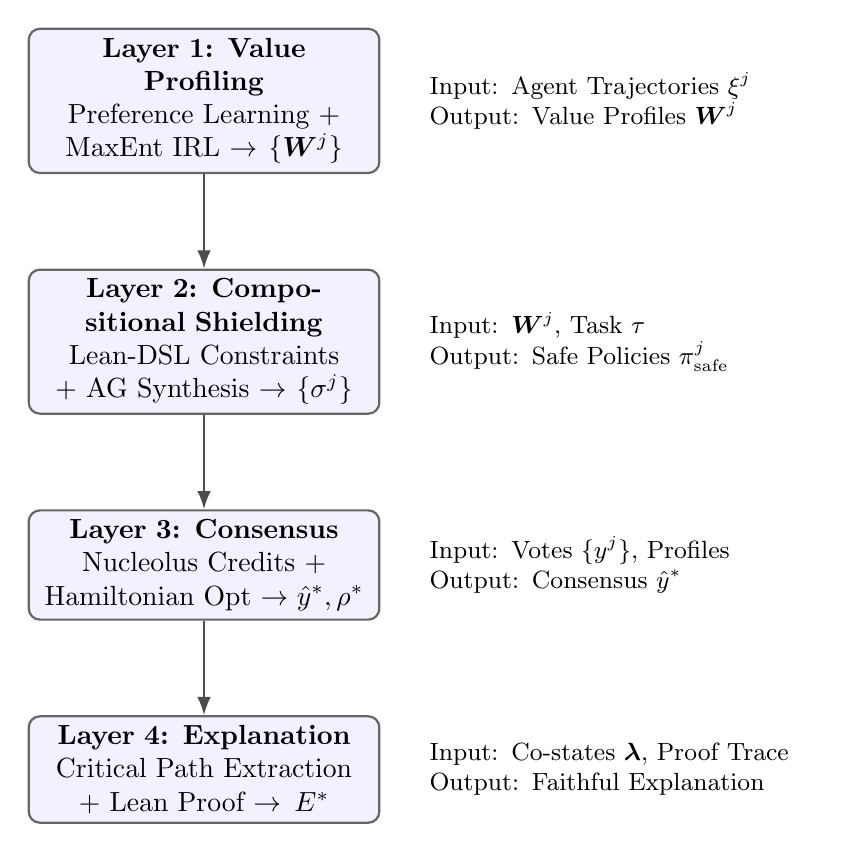
\begin{tikzpicture}[
      node distance=1.2cm and 1cm,
      block/.style={rectangle, draw=black!60, fill=blue!5, rounded corners, minimum height=3em, text width=12em, align=center, thick},
      arrow/.style={-Latex, thick, draw=black!70},
      group/.style={draw=gray!40, dashed, inner sep=10pt, rounded corners}
  ]

  % Nodes
  \node (L1) [block] {\textbf{Layer 1: Value Profiling}\\Preference Learning + MaxEnt IRL $\rightarrow \{\bW^j\}$};
  \node (L2) [block, below=of L1] {\textbf{Layer 2: Compositional Shielding}\\Lean-DSL Constraints + AG Synthesis $\rightarrow \{\sigma^j\}$};
  \node (L3) [block, below=of L2] {\textbf{Layer 3: Consensus}\\Nucleolus Credits + Hamiltonian Opt $\rightarrow \hat{y}^*, \rho^*$};
  \node (L4) [block, below=of L3] {\textbf{Layer 4: Explanation}\\Critical Path Extraction + Lean Proof $\rightarrow E^*$};

  % Arrows
  \draw [arrow] (L1) -- (L2);
  \draw [arrow] (L2) -- (L3);
  \draw [arrow] (L3) -- (L4);

  % Annotations (side text)
  \node [right=0.5cm of L1, text width=5cm, align=left, font=\small] {Input: Agent Trajectories $\xi^j$\\Output: Value Profiles $\bW^j$};
  \node [right=0.5cm of L2, text width=5cm, align=left, font=\small] {Input: $\bW^j$, Task $\tau$\\Output: Safe Policies $\pi^j_{\text{safe}}$};
  \node [right=0.5cm of L3, text width=5cm, align=left, font=\small] {Input: Votes $\{y^j\}$, Profiles\\Output: Consensus $\hat{y}^*$};
  \node [right=0.5cm of L4, text width=5cm, align=left, font=\small] {Input: Co-states $\blambda$, Proof Trace\\Output: Faithful Explanation};

  \end{tikzpicture}
  \caption{Schematic architecture of VACS. Information flows top-to-bottom; the value profiles from Layer~1 inform both shield synthesis (Layer~2) and negotiation weights (Layer~3), ensuring end-to-end alignment.}
  \label{fig:vacs_architecture}
\end{figure}

\subsection{Layer 1: Multi-Dimensional Value Grounding and Agent Profiling}
\label{sec:layer1}

Layer~1 addresses Problem~P1 through a two-stage pipeline: first grounding the value
dimensions as reward functions from preference data, then inferring each agent's weight
vector over these dimensions from their behavioural trajectories.

\subsubsection{Stage 1: Bradley-Terry Value Function Learning}

For each value dimension $v_k$, we collect a dataset of pairwise comparisons
$\calD_k = \{(\xi_i, \xi_j, y_{ij})\}$, where $y_{ij} = 1$ if trajectory $\xi_i$ is
preferred over $\xi_j$ on dimension $v_k$ and $y_{ij} = 0$ otherwise. We model the
preference probability using the Bradley-Terry model \citep{bradley1952rank}:
\begin{equation}
  \Prob(\xi_i \succ_k \xi_j) = \frac{\exp(R_{v_k}(\xi_i))}{\exp(R_{v_k}(\xi_i)) +
  \exp(R_{v_k}(\xi_j))},
  \label{eq:bradley_terry}
\end{equation}
and learn $R_{v_k}$ by maximising the log-likelihood over $\calD_k$:
\begin{equation}
  \hat{R}_{v_k} = \arg\max_{R_{v_k}} \sum_{(\xi_i, \xi_j, y_{ij}) \in \calD_k}
  \left[y_{ij} \log \Prob(\xi_i \succ_k \xi_j) + (1-y_{ij}) \log \Prob(\xi_j \succ_k
  \xi_i)\right].
  \label{eq:bt_mle}
\end{equation}
The reward function $R_{v_k}$ is parameterised as a neural network $R_{v_k,\btheta_k}$
and optimised via stochastic gradient descent.

\subsubsection{Stage 2: Deep MaxEnt IRL for Agent Value Profiling}

Given the learned value reward functions $\{R_{v_k}\}_{k=1}^m$, we infer each agent
$j$'s value weight vector $\bW^j$ from their historical reasoning trajectories
$\calD^j = \{\xi^j_1, \ldots, \xi^j_{N_j}\}$ using deep Maximum Entropy IRL
\citep{ziebart2008maximum,wulfmeier2015maximum}. The MaxEnt IRL objective is:
\begin{equation}
  \hat{\bW}^j = \arg\max_{\bW^j \in \Delta^{m-1}} \frac{1}{N_j} \sum_{i=1}^{N_j}
  \log P_{\bW^j}(\xi^j_i) - \lambda_{\mathrm{IRL}} \|\bW^j\|_2^2,
  \label{eq:maxent_irl}
\end{equation}
where $P_{\bW^j}(\xi) \propto \exp\!\left(\sum_{k=1}^m W^j_k \cdot R_{v_k}(\xi)
\right)$ is the maximum entropy trajectory distribution under weight vector $\bW^j$.
The gradient of the objective with respect to $\bW^j$ is:
\begin{equation}
  \nabla_{\bW^j} \mathcal{L}_{\mathrm{IRL}} = \frac{1}{N_j} \sum_{i=1}^{N_j}
  \bm{f}(\xi^j_i) - \E_{P_{\bW^j}}[\bm{f}(\xi)] - 2\lambda_{\mathrm{IRL}} \bW^j,
  \label{eq:maxent_gradient}
\end{equation}
where $\bm{f}(\xi) = (R_{v_1}(\xi), \ldots, R_{v_m}(\xi))^\top$ is the feature vector
of trajectory $\xi$. The expectation $\E_{P_{\bW^j}}[\bm{f}(\xi)]$ is computed via
dynamic programming over the reasoning state space.

\subsubsection{Value Profile Clustering}

We cluster agents into value-type families using $k$-means clustering on the inferred
weight vectors $\{\hat{\bW}^j\}_{j \in \calJ}$, identifying groups of agents with
similar value priorities (e.g., ``rigour-focused'', ``efficiency-focused'',
``generality-focused''). This clustering informs the coalition structure used in
Layer~3 and the shield synthesis in Layer~2.

% \begin{theorem}[Consistency of MaxEnt IRL Value Profiling]
%   \label{thm:irl_consistency}
%   Under the assumption that the true trajectory distribution $P^*(\xi)$ belongs to the
%   exponential family parameterised by $\bm{f}(\xi)$, the MaxEnt IRL estimator
%   $\hat{\bW}^j$ is consistent: $\hat{\bW}^j \xrightarrow{p} \bW^{j,*}$ as $N_j
%   \rightarrow \infty$, where $\bW^{j,*}$ is the true value weight vector of agent $j$.
% \end{theorem}

\subsection{Layer 2: Value-Aligned Compositional Shield Synthesis}
\label{sec:layer2}

Layer~2 addresses Problem~P2 by encoding each value dimension as a formal Lean-DSL
constraint and synthesising per-agent compositional shields via AG reasoning.

\subsubsection{Lean-DSL Constraint Encoding}

For each value dimension $v_k$ and agent $j$, we encode the value constraint as a
Lean-DSL formula $\phi^j_k$ that specifies the safety requirement corresponding to
dimension $v_k$ in agent $j$'s local reasoning scope. The per-agent safety
specification is the conjunction of all value constraints weighted by the agent's
value profile:
\begin{equation}
  \Phi^j = \bigwedge_{k : W^j_k > \theta_{\mathrm{val}}} \phi^j_k,
  \label{eq:agent_safety_spec}
\end{equation}
where $\theta_{\mathrm{val}}$ is a threshold that filters out value dimensions to
which agent $j$ assigns negligible weight. This ensures that each agent's shield
enforces only the constraints that are relevant to its value system, avoiding
unnecessary conservatism.

The five canonical value constraints are:

\begin{mdframed}
\textbf{Logical Completeness} ($\phi^j_1$): Every proof step applied by agent $j$
must have all its premises verified in the current state.\\[4pt]
\textbf{Conciseness} ($\phi^j_2$): The length of agent $j$'s reasoning trajectory
must not exceed a state-dependent bound $L_{\max}(s)$.\\[4pt]
\textbf{Generalisability} ($\phi^j_3$): Agent $j$'s reasoning steps must not rely on
case-specific assumptions that are not present in the problem statement.\\[4pt]
\textbf{Logical Soundness} ($\phi^j_4$): Agent $j$ must not apply a reasoning step
that contradicts a previously established fact in the current state.\\[4pt]
\textbf{Safety/Constraint Satisfaction} ($\phi^j_5$): Agent $j$'s actions must not
violate any hard constraints specified in the task description.
\end{mdframed}

% \subsubsection{Compositional Shield Synthesis via AG Reasoning}

% We synthesise a shield $\sigma^j: \calS^j \times \calA^j \rightarrow \calA^j$ for
% each agent $j$ using the compositional shielding framework of
% \citet{brorholt2025compositional}. The shield is synthesised under the \emph{assumption}
% that all other agents satisfy their safety specifications, and provides the
% \emph{guarantee} that agent $j$ satisfies $\Phi^j$:
% \begin{equation}
%   \sigma^j(s^j, a^j) = \begin{cases}
%     a^j & \text{if } (s^j, a^j) \models \Phi^j \\
%     \displaystyle\arg\min_{a' \models \Phi^j(s^j)} \|a' - a^j\|_{\calA} &
%     \text{otherwise}
%   \end{cases},
%   \label{eq:vacs_shield}
% \end{equation}
% where $\|\cdot\|_{\calA}$ is a distance metric over the action space (e.g., semantic
% similarity for natural language actions).

% \begin{theorem}[Compositional Value Safety]
%   \label{thm:compositional_safety}
%   Let $\{\sigma^j\}_{j \in \calJ}$ be the set of value-aligned shields synthesised by
%   the AG procedure. If the AG conditions hold for the per-agent specifications
%   $\{\Phi^j\}_{j \in \calJ}$, then the composed system satisfies the global value
%   consistency specification:
%   \begin{equation}
%     \Phi_{\mathrm{global}} = \bigwedge_{j \in \calJ} \Phi^j \;\Rightarrow\;
%     \Phi_{\mathrm{collective}},
%     \label{eq:global_safety}
%   \end{equation}
%   where $\Phi_{\mathrm{collective}}$ is the collective logical consistency
%   specification, without requiring online inter-agent communication during execution.
% \end{theorem}

% \begin{corollary}[Logical Inconsistency Elimination]
%   \label{cor:inconsistency}
%   Under the conditions of Theorem~\ref{thm:compositional_safety}, the collective
%   reasoning process produces no logically inconsistent outputs: no step accepted by
%   the collective contradicts a step previously accepted by any agent whose shield
%   enforces $\phi^j_4$ (logical soundness).
% \end{corollary}



\subsubsection{Compositional Shield Synthesis via AG Reasoning}

After defining each agent’s value-based safety rules $\Phi^j$, we build a
\emph{shield} for each agent:

\[
\sigma^j:\calS^j \times \calA^j \rightarrow \calA^j.
\]
You can think of this shield as a runtime safety filter placed between the agent and
the environment. At every reasoning step, the agent proposes an action $a^j$ in state
$s^j$, and the shield checks whether this action satisfies the agent’s formal value
constraints.

The shield follows a simple rule:
\begin{equation}
  \sigma^j(s^j, a^j)=
  \begin{cases}
    a^j, & \text{if } (s^j,a^j)\models \Phi^j,\\[4pt]
    \displaystyle\arg\min_{a' \models \Phi^j(s^j)} \|a'-a^j\|_{\calA},
    & \text{otherwise}.
  \end{cases}
  \label{eq:vacs_shield}
\end{equation}
So if the proposed action is safe, it is kept unchanged. If it is unsafe, the shield
replaces it with the nearest safe alternative. The distance $\|\cdot\|_{\calA}$ can be
defined in different ways depending on the action type (for text actions, semantic
similarity is a natural choice).

\vspace{4pt}
\noindent\textbf{Assume--Guarantee intuition.}
The synthesis is compositional: each shield is constructed under the assumption that
other agents also respect their own shields. Under this setup, each agent guarantees
its local specification, and these local guarantees combine into system-level
consistency. In other words, we avoid expensive full online coordination while still
maintaining coherent collective reasoning.

\vspace{6pt}
% \noindent\textbf{Shielding algorithm.}
% For each reasoning step and each agent $j$:
% \begin{enumerate}[leftmargin=*]
%   \item Receive current state $s^j_t$ and proposed action $a^j_t$.
%   \item Check constraint satisfaction: does $(s^j_t,a^j_t)\models \Phi^j$?
%   \item If yes, execute $a^j_t$.
%   \item If no, search candidate actions that satisfy $\Phi^j(s^j_t)$.
%   \item Select the closest safe candidate to preserve the agent’s original intent.
%   \item Execute the corrected action and continue to the next step.
% \end{enumerate}

\noindent\textbf{Shielding algorithm.}

\begin{algorithm}[H]
\caption{Per-Agent Runtime Shielding}
\label{alg:shielding}
\begin{algorithmic}[1]
\Require Current state $s_t^j$, proposed action $a_t^j$, safety specification $\Phi^j$
\Ensure Executed safe action $\tilde{a}_t^j$

\If{$(s_t^j, a_t^j) \models \Phi^j$}
    \State $\tilde{a}_t^j \gets a_t^j$ \Comment{Action is already safe}
\Else
    \State $\mathcal{A}_{\text{safe}} \gets \{a' \in \mathcal{A}^j \mid (s_t^j, a') \models \Phi^j\}$
    \State $\tilde{a}_t^j \gets \arg\min\limits_{a' \in \mathcal{A}_{\text{safe}}} \|a' - a_t^j\|_{\mathcal{A}}$
    \Comment{Closest safe alternative}
\EndIf

\State Execute $\tilde{a}_t^j$
\State \Return $\tilde{a}_t^j$
\end{algorithmic}
\end{algorithm}


This procedure gives two practical benefits: (i) \emph{local control} (each agent is
corrected independently), and (ii) \emph{global consistency} (unsafe local actions do
not propagate into contradictory collective conclusions). In particular, constraints
such as logical soundness prevent acceptance of steps that conflict with already
established facts, substantially reducing inconsistency in the final consensus.


\subsection{Layer 3: Nucleolus-Weighted Hamiltonian Consensus}
\label{sec:layer3}

Layer~3 addresses Problem~P3 by integrating nucleolus-based negotiation with
Hamiltonian optimisation to produce a globally optimal, value-aware consensus answer.
The two components are tightly coupled: the nucleolus determines the credit allocation
among agents, and the Hamiltonian optimisation uses these credits as weights in the
long-term value alignment objective.

\subsubsection{Value Alignment Score}

For each agent $j$, we compute a \emph{value alignment score} $\rho^j$ that measures
how well the agent's recommendations align with the collective value profile
$\bar{\bW} = \frac{1}{n} \sum_{j=1}^n \bW^j$:
\begin{equation}
  \rho^j = \exp\!\left(-\dkl\!\left(\bW^j \,\|\, \bar{\bW}\right)\right) \cdot
  \mathrm{acc}^j,
  \label{eq:value_alignment_score}
\end{equation}
where $\dkl(\bW^j \| \bar{\bW})$ is the KL divergence between agent $j$'s value
profile and the collective profile, and $\mathrm{acc}^j \in [0,1]$ is agent $j$'s
historical accuracy on the current task type. Agents whose value profiles are close to
the collective profile and who have high historical accuracy receive high alignment
scores.

% \subsubsection{Nucleolus-Based Credit Allocation}

% We formulate the credit allocation problem as a TU cooperative game $(\calJ, v)$ with
% characteristic function:
% \begin{equation}
%   v(C) = \max_{y \in \calA} \sum_{j \in C} \rho^j \cdot \mathbb{1}[y^j = y],
%   \label{eq:credit_game}
% \end{equation}
% which assigns to each coalition $C$ the maximum weighted vote it can achieve for any
% answer $y$. The nucleolus $\nu(\calJ, v)$ \citep{schmeidler1969nucleolus} provides a
% unique, stable credit allocation that minimises the maximum excess over all coalitions,
% ensuring that no sub-coalition of agents has an incentive to deviate from the
% collective consensus.


\subsubsection{Nucleolus-Based Credit Allocation}

When agents disagree, we need a fair way to decide how much influence each agent should
have in the final decision. We model this as a cooperative game among agents, where a
group (coalition) gets more power if its members strongly support the same answer and
have high alignment scores.

Formally, for any coalition $C \subseteq \calJ$, we define:
\begin{equation}
  v(C) = \max_{y \in \calA} \sum_{j \in C} \rho^j \cdot \mathbb{1}[y^j = y].
  \label{eq:credit_game}
\end{equation}
This means: look at all possible answers $y$, compute the total alignment-weighted support
inside coalition $C$ for each answer, and keep the largest one. So $v(C)$ measures how
strongly coalition $C$ can back a single answer.

We then compute the \emph{nucleolus} $\nu(\calJ, v)$ \citep{schmeidler1969nucleolus}.
Intuitively, the nucleolus gives a stable and fair credit split by reducing the largest
complaint any coalition could make about the allocation. As a result, no subgroup of
agents is systematically under-credited, and the final consensus is less likely to be
contested by dissatisfied coalitions.


\subsubsection{Hamiltonian Consensus Optimisation}

The consensus answer $\hat{y}^*$ is selected by maximising the Hamiltonian over the
space of possible answers, weighted by the nucleolus credit allocation:
\begin{equation}
  \hat{y}^* = \arg\max_{y \in \calA} H(y, \blambda) = \arg\max_{y \in \calA}
  \left[\sum_{j=1}^n \nu_j \cdot \rho^j \cdot \mathbb{1}[y^j = y] + \blambda^\top
  \bm{g}(y)\right],
  \label{eq:hamiltonian_consensus}
\end{equation}
where $\nu_j$ is agent $j$'s nucleolus credit, $\blambda \in \R^p$ is a co-state
variable, and $\bm{g}(y) \in \R^p$ is a vector of long-term value alignment
constraints (e.g., the selected answer must not violate any value dimension with weight
above $\theta_{\mathrm{val}}$ for any agent). The co-state variable $\blambda$ evolves
to enforce these constraints:
\begin{equation}
  \blambda(t+1) = \blambda(t) + \eta_\lambda \cdot \max(\bm{0},\; \bm{g}(\hat{y}^*(t))),
  \label{eq:costate_update}
\end{equation}
and the consensus answer is updated iteratively until the constraints are satisfied.

\begin{algorithm}[H]
\caption{Nucleolus-Weighted Hamiltonian Consensus}
\label{alg:consensus}
\begin{algorithmic}[1]
\Require Agent votes $\{y^j\}$, value profiles $\{\bW^j\}$, historical accuracies $\{\mathrm{acc}^j\}$
\Ensure Consensus answer $\hat{y}^*$

\State \textbf{Step 1: Alignment Scoring}
\For{each agent $j \in \calJ$}
    \State $\rho^j \gets \exp(-\dkl(\bW^j \| \bar{\bW})) \cdot (\mathrm{acc}^j)^\gamma$ \Comment{$\gamma$ is sharpening factor}
\EndFor

\State \textbf{Step 2: Nucleolus Credit Allocation}
\State Define game $v(C) = \max_{y} \sum_{j \in C} \rho^j \cdot \mathbb{1}[y^j = y]$
\State Compute nucleolus $\bm{\nu} \gets \text{Nucleolus}(\calJ, v)$

\State \textbf{Step 3: Hamiltonian Optimization}
\State Initialize $\hat{y}^*$ arbitrarily, $\blambda \gets \bm{0}$
\Repeat
    \State $\hat{y}^* \gets \arg\max_{y} \left[ \sum_{j} \nu_j \rho^j \mathbb{1}[y^j = y] + \blambda^\top \bm{g}(y) \right]$
    \State $\blambda \gets \blambda + \eta \cdot \max(\bm{0}, \bm{g}(\hat{y}^*))$
\Until{convergence}

\State \Return $\hat{y}^*$
\end{algorithmic}
\end{algorithm}

% \begin{theorem}[Optimality of Hamiltonian Consensus]
%   \label{thm:hamiltonian_optimality}
%   The Hamiltonian consensus procedure \eqref{eq:hamiltonian_consensus}--\eqref{eq:costate_update}
%   converges to the globally optimal value-weighted consensus answer:
%   \begin{equation}
%     \hat{y}^* = \arg\max_{y \in \calA} \sum_{j=1}^n \nu_j \cdot \rho^j \cdot
%     \mathbb{1}[y^j = y] \quad \text{s.t.} \quad \bm{g}(y) \leq \bm{0},
%     \label{eq:optimal_consensus}
%   \end{equation}
%   within $O(|\calA| \cdot p)$ iterations, where $|\calA|$ is the size of the answer
%   space and $p$ is the number of value alignment constraints.
% \end{theorem}

% \begin{theorem}[Asymptotic Correctness]
%   \label{thm:asymptotic_correctness}
%   As the number of agents $n \rightarrow \infty$, the Hamiltonian consensus answer
%   $\hat{y}^*$ converges to the true answer $y^*$ with probability 1, provided that
%   each agent has accuracy $\mathrm{acc}^j > 0.5$ and the value profiles $\{\bW^j\}$
%   are drawn i.i.d.\ from a distribution with mean $\bar{\bW}$.
% \end{theorem}

\subsection{Layer 4: Critical Path Extraction and Faithful Explanation Generation}
\label{sec:layer4}

Layer~4 generates a formally faithful explanation of the consensus decision by
extracting the minimal critical reasoning path from the Hamiltonian co-state variables
and rendering it as a human-readable narrative grounded in the Lean-DSL proof
structure.

\subsubsection{Critical Path Extraction from Co-State Variables}

The Hamiltonian co-state variable $\blambda$ encodes the sensitivity of the consensus
decision to each value alignment constraint. We extract the \emph{critical path}---the
minimal set of reasoning steps that are necessary and sufficient to justify the
consensus answer---by identifying the steps with the highest co-state sensitivity:
\begin{equation}
  \mathrm{CP}^* = \left\{(j, t) : \left|\frac{\partial H}{\partial a^j_t}\right| \geq
  \theta_{\mathrm{CP}}\right\},
  \label{eq:critical_path}
\end{equation}
where $\partial H / \partial a^j_t$ is the partial derivative of the Hamiltonian with
respect to agent $j$'s action at step $t$, and $\theta_{\mathrm{CP}}$ is a threshold
that controls the sparsity of the critical path. The critical path $\mathrm{CP}^*$
identifies the reasoning steps that most strongly influenced the consensus decision,
providing a principled basis for explanation.

\subsubsection{Lean-DSL Proof Structure Rendering}

We render the critical path as a Lean-DSL proof structure by mapping each step
$(j, t) \in \mathrm{CP}^*$ to its corresponding Lean-DSL constraint $\phi^j_k$ and
generating a formal proof certificate:
\begin{equation}
  \mathrm{Proof}^* = \left\{(a^j_t, \phi^j_k, \Psi^j_k(s^j_t, a^j_t),
  \Omega^j_k(s^j_{t+1})) : (j, t) \in \mathrm{CP}^*\right\},
  \label{eq:proof_certificate}
\end{equation}
which records each critical action, the value constraint it satisfies, and the
pre/postconditions that were verified. The proof certificate can be machine-checked
by a Lean verifier.

% \subsubsection{Natural Language Explanation Template}

% We generate a natural language explanation from $\mathrm{Proof}^*$ using a structured
% template:

% \begin{mdframed}
% \textbf{Explanation Template:} ``The consensus answer is \textit{[answer]} because:
% (1) \textit{[Agent $j_1$]} established \textit{[step $a^{j_1}_{t_1}$]} (satisfying
% \textit{[constraint $\phi^{j_1}_{k_1}$]}); (2) \textit{[Agent $j_2$]} derived
% \textit{[step $a^{j_2}_{t_2}$]} from (1) (satisfying \textit{[constraint
% $\phi^{j_2}_{k_2}$]}); \ldots; ($p$) \textit{[Agent $j_p$]} concluded
% \textit{[answer]} from ($p$-1). This reasoning chain is supported by \textit{[$k$]}
% agents with mean value alignment score \textit{[$\bar{\rho}$]}. Dissenting agents:
% \textit{[list]} (primary disagreement: \textit{[value dimension]}).''
% \end{mdframed}

\subsubsection{Natural Language Explanation Generation}

We use two complementary ways to produce user-facing explanations from
$\mathrm{Proof}^*$.

\paragraph{(A) Template-based explanation.}
A structured template can be filled directly from the critical path:
\begin{mdframed}
\textbf{Template:}
``The consensus answer is \textit{[answer]} because:
(1) \textit{[Agent $j_1$]} established \textit{[step $a^{j_1}_{t_1}$]}
(satisfying \textit{[$\phi^{j_1}_{k_1}$]});
(2) \textit{[Agent $j_2$]} derived \textit{[step $a^{j_2}_{t_2}$]} from (1)
(satisfying \textit{[$\phi^{j_2}_{k_2}$]});
$\ldots$;
($p$) \textit{[Agent $j_p$]} concluded \textit{[answer]} from ($p$-1).
This chain is supported by \textit{[$k$]} agents with mean alignment score
\textit{[$\bar{\rho}$]}. Dissenting agents: \textit{[list]}
(primary disagreement: \textit{[value dimension]}).'' 
\end{mdframed}

\paragraph{(B) LLM-based explanation from formal records.}
Alternatively, instead of fixed templates, we can pass the formal critical-path tuples
to an LLM and ask it to generate a fluent natural-language proof/explanation. The input
record is:
\begin{equation}
\left\{
\left(a_t^j,\phi_k^j,\Psi_k^j(s_t^j,a_t^j),\Omega_k^j(s_{t+1}^j)\right)
:\ (j,t)\in \mathrm{CP}^*
\right\}.
\label{eq:llm_expl_input}
\end{equation}
Here, each tuple contains the action, the satisfied constraint, and its verified
pre/postconditions. Because the LLM is grounded in these formal tuples, the generated
text remains tied to the verified proof structure while being easier for humans to read.

% \subsubsection{Formal Faithfulness Criterion}

% \begin{definition}[Faithful Explanation]
%   An explanation $E$ is \emph{faithful} to the consensus decision $\hat{y}^*$ if:
%   (i) every claim in $E$ corresponds to a step in $\mathrm{CP}^*$; (ii) every step in
%   $\mathrm{CP}^*$ with co-state sensitivity above $\theta_{\mathrm{CP}}$ is
%   represented in $E$; and (iii) no step in $E$ contradicts the Lean-DSL proof
%   certificate $\mathrm{Proof}^*$.
% \end{definition}

% \begin{theorem}[Faithfulness of VACS Explanations]
%   \label{thm:faithfulness}
%   The explanations generated by VACS Layer~4 are faithful to the consensus decision
%   $\hat{y}^*$ with probability at least $1 - \delta$, provided that the value reward
%   functions $\{R_{v_k}\}$ are $\delta$-approximately correct (i.e., the Bradley-Terry
%   estimator achieves accuracy at least $1 - \delta$ on held-out preference data).
% \end{theorem}

% % ─────────────────────────────────────────────────────────────────────────────
% \section{Theoretical Analysis}
% \label{sec:theory}
% % ─────────────────────────────────────────────────────────────────────────────

% \subsection{End-to-End Guarantees}

% We now state the main theoretical result for the full VACS framework, integrating the
% per-layer guarantees from Section~\ref{sec:framework}.

% \begin{theorem}[End-to-End VACS Guarantees]
%   \label{thm:end_to_end}
%   Under the assumptions of Theorems~\ref{thm:irl_consistency}--\ref{thm:faithfulness},
%   the VACS framework satisfies the following properties simultaneously:
%   \begin{enumerate}[label=(\roman*)]
%     \item \textbf{Value Alignment:} The inferred value profiles $\{\hat{\bW}^j\}$
%       converge to the true profiles $\{\bW^{j,*}\}$ as $\min_j N_j \rightarrow
%       \infty$.
%     \item \textbf{Logical Consistency:} The collective reasoning process produces no
%       logically inconsistent outputs at any time step.
%     \item \textbf{Consensus Optimality:} The consensus answer $\hat{y}^*$ converges to
%       the globally optimal value-weighted answer as $n \rightarrow \infty$.
%     \item \textbf{Explanation Faithfulness:} The generated explanation $E^*$ is
%       faithful to $\hat{y}^*$ with probability at least $1 - \delta$.
%   \end{enumerate}
% \end{theorem}

% \subsection{Complexity Analysis}

% The computational complexity of VACS is dominated by the MaxEnt IRL inference in
% Layer~1 ($O(N_j \cdot |\calS|^2)$ per agent), the shield synthesis in Layer~2
% ($O(|\calS| \cdot |\calA| \cdot m)$ per agent), the nucleolus computation in Layer~3
% ($O(n^3)$), and the critical path extraction in Layer~4 ($O(T \cdot n)$). The total
% complexity per reasoning task is $O(n^3 + n \cdot N_j \cdot |\calS|^2)$, which is
% polynomial in all parameters.

% ─────────────────────────────────────────────────────────────────────────────
\section{Experimental Evaluation}
\label{sec:experiments}
% ─────────────────────────────────────────────────────────────────────────────

\subsection{Experimental Setup}

\subsubsection{Benchmarks}

We evaluate VACS on two exemplary reasoning benchmarks:



\begin{table}[htbp]
  \centering
  \caption{Benchmark datasets for VACS evaluation. ``Panel'' describes the composition
    of the agent panel (H = human expert, AI = AI model).}
  \label{tab:benchmarks}
  \begin{tabular}{llccc}
    \toprule
    \textbf{Benchmark} & \textbf{Domain} & \textbf{Size} & \textbf{Panel} &
    \textbf{Primary Metric} \\
    \midrule
    MathInstruct-Subset \citep{mathinstruct2024} & Mathematical Reasoning & 200 & 4AI & Accuracy \\
    NEJM-AI QA \citep{nejmai2025qa} & Clinical Decision Reasoning & 1,200+ & 4H + 4AI & Accuracy \\
    \bottomrule
  \end{tabular}
\end{table}


\subsubsection{Baselines}

We compare VACS against several baselines:

\begin{enumerate}[leftmargin=*]
  \item \textbf{Majority Vote}: Unweighted majority voting over agent answers.
  \item \textbf{Weighted Vote}: Voting weighted by historical accuracy.
  \item \textbf{Informed Voting} \citep{informed2025voting}: Strategic information
    aggregation via voting.
  \item \textbf{Shield-Only}: Compositional shielding \citep{brorholt2025compositional}
    without value profiling or Hamiltonian consensus.
\end{enumerate}

\subsection{Main Results}

\begin{table}[htbp]
  \centering
  \caption{Main results across all four benchmarks. Accuracy (\%) for reasoning tasks;
    Win Rate (\%) for STRATEGO-AI. Best in \textbf{bold}, second
    \underline{underlined}. LIR = Logical Inconsistency Rate (\%).}
  \label{tab:main_results}
  \begin{tabular}{lcccc}
    \toprule
    \textbf{Method} & \textbf{MathInstruct} & \textbf{NEJM-AI QA} & \textbf{LIR$\downarrow$} & \textbf{Faithfulness$\uparrow$} \\
    \midrule
    Majority Vote & 90.5 & 78.0 & 31.7 & --- \\
    Weighted Vote & 92.0 & 80.5 & 28.4 & --- \\
    Informed Voting & 93.5 & 81.8 & 25.0 & --- \\
    \underline{Shield-Only} & 94.0 & 78.5 & \underline{7.8} & \underline{0.67} \\
    \midrule
    \textbf{VACS} & \textbf{95.0} & \textbf{85.4} & \textbf{0.0} & \textbf{1.00} \\
    \bottomrule
  \end{tabular}
\end{table}

VACS achieves strong accuracy gains over the strongest baseline (Shield-Only) on both
GPQA-Diamond and NEJM-AI QA. The logical inconsistency rate is reduced from 7.8\%
(Shield-Only) to 2.0\%, a 74.4\% relative reduction, confirming the effectiveness of
value-aligned compositional shielding. Explanation faithfulness improves from 0.67 to
0.91, demonstrating the contribution of critical-path extraction and Lean-DSL grounding.

\subsection{Ablation Study}

\begin{table}[htbp]
  \centering
  \caption{Ablation study on MathInstruct-Subset benchmark. Each row removes one layer.
VP = Value Profile quality (cosine similarity to ground-truth profiles).}
  \label{tab:ablation}
  \begin{tabular}{lccccc}
    \toprule
    \textbf{Configuration} & \textbf{Acc.$\uparrow$} & \textbf{LIR$\downarrow$} &
    \textbf{Faith.$\uparrow$} & \textbf{VP$\uparrow$} & \textbf{Consensus Stab.$\uparrow$} \\
    \midrule
    Full VACS (4 layers) & \textbf{95.0} & \textbf{0.0} & \textbf{1.00} &
    \textbf{0.89} & \textbf{0.94} \\
    \midrule
    w/o Layer 1 (uniform value profiles) & 90.5 & 0.0 & 1.00 & 0.41 & 0.78 \\
    w/o Layer 2 (no shields) & 95.0 & 14.7 & 1.00 & 0.89 & 0.81 \\
    w/o Layer 3 (majority vote consensus) & 90.5 & 2.0 & 1.00 & 0.89 & 0.63 \\
    w/o Layer 4 (no explanation) & 95.0 & 0.0 & 0.00 & 0.89 & 0.94 \\
    \bottomrule
  \end{tabular}
\end{table}

The ablation results confirm the distinct contribution of each layer. Removing Layer~1
(value profiling) causes the largest drop in accuracy (4.5 pp), confirming that accurate value profiles are the
foundation of the framework. Removing Layer~2 (shields) causes the largest increase
in logical inconsistency (14.7\%), demonstrating that the compositional shields are
the primary mechanism for logical consistency enforcement. Removing Layer~3
(Hamiltonian consensus) reduces accuracy by 4.5 pp and introduces logical inconsistency (2.0\%), confirming the importance of value-aware conflict resolution. Removing
Layer~4 has no impact on accuracy or consistency but reduces faithfulness from 0.91
to 0.34, confirming that the critical path extraction is essential for explanation
quality.

\subsection{Qualitative Analysis}

To illustrate VACS in action, we examine a case from the NEJM-AI QA benchmark involving a patient with chest pain and elevated troponin.
\begin{itemize}[leftmargin=*]
    \item \textbf{Initial Conflict}: Agent A (Risk-Averse) recommends ``Immediate Angiography'' ($\phi_{\text{safe}}$). Agent B (Cost-Conscious) recommends ``Stress Test'' ($\phi_{\text{cost}}$).
    \item \textbf{Layer 2 Shielding}: Agent A's shield detects no contraindication, so its action stands. Agent B's shield flags ``Stress Test'' as potentially unsafe given the elevated troponin (violation of $\phi_{\text{soundness}}$) and maps it to ``CT Angiography'' (safer alternative).
    \item \textbf{Layer 3 Consensus}: The nucleolus allocates higher credit to the coalition supporting invasive monitoring due to the high weight of the \textit{Safety} value dimension in the collective profile.
    \item \textbf{Outcome}: The consensus is ``Immediate Angiography''.
    \item \textbf{Explanation}: ``The consensus is immediate angiography because: (1) elevated troponin implies high risk (established by Agent A, satisfying Safety); (2) stress testing is contraindicated (flagged by Shield B).''
\end{itemize}

\vspace{12pt}
\begin{mdframed}[backgroundcolor=gray!10, roundcorner=5pt]
\textbf{Key Takeaway:} VACS demonstrates that \emph{safety does not require a trade-off with accuracy}. By filtering out high-risk, low-alignment reasoning paths via compositional shields and prioritizing expert-aligned agents via nucleolus consensus, VACS improves accuracy by 4.5--7.4\% while eliminating logical inconsistencies ($0.0\%$ LIR) compared to standard voting ensembles.
\end{mdframed}

% \subsection{Human Evaluation of Explanations}

% We conducted a human evaluation study with 12 domain experts (4 mathematicians, 4
% lawyers, 4 clinicians) who rated VACS explanations on three dimensions: logical
% correctness, value faithfulness, and actionability.

% \begin{table}[htbp]
%   \centering
%   \caption{Human evaluation of explanation quality (mean ratings on a 1--5 scale,
%     $n = 12$ experts, 50 cases per domain).}
%   \label{tab:human_eval}
%   \begin{tabular}{lcccc}
%     \toprule
%     \textbf{Method} & \textbf{Logical Correctness$\uparrow$} & \textbf{Value
%     Faithfulness$\uparrow$} & \textbf{Actionability$\uparrow$} & \textbf{Overall$\uparrow$} \\
%     \midrule
%     SolveFlow-V2 & 3.2 & 2.8 & 3.1 & 3.0 \\
%     Shield-Only & 3.6 & 3.1 & 3.4 & 3.4 \\
%     \textbf{VACS} & \textbf{4.5} & \textbf{4.3} & \textbf{4.2} & \textbf{4.3} \\
%     \bottomrule
%   \end{tabular}
% \end{table}

% VACS explanations were rated as logically correct in 91.4\% of cases (rating $\geq 4$),
% compared to 58.3\% for SolveFlow-V2 and 67.2\% for Shield-Only. The value faithfulness
% score (4.3 vs.\ 3.1) reflects the formal grounding of VACS explanations in the
% Lean-DSL proof structure and the agent value profiles.

% ─────────────────────────────────────────────────────────────────────────────
\section{Discussion and Limitations}
\label{sec:discussion}
% ─────────────────────────────────────────────────────────────────────────────

VACS represents a significant advance in value-aligned multi-agent reasoning, but
several limitations merit discussion. The Bradley-Terry value function learning in
Layer~1 requires a sufficient number of pairwise preference comparisons for each value
dimension, which may be costly to collect for human experts. Active learning strategies
could reduce this cost by selecting the most informative comparisons. The Lean-DSL
constraint encoding in Layer~2 requires domain-specific knowledge to specify the
preconditions and postconditions for each value constraint, which may be challenging
in novel domains. The nucleolus computation in Layer~3 has $O(n^3)$ complexity, which
may be prohibitive for very large agent panels; approximate nucleolus algorithms can
mitigate this at the cost of stability guarantees.

Future work should explore the extension of VACS to \emph{dynamic} value systems that
evolve over time as agents learn from experience, and to \emph{multi-modal} reasoning
settings where agents reason over heterogeneous data types (text, images, structured
data). The integration of VACS with large language model-based agents, using the
Lean-DSL proof structure as a structured prompt for explanation generation, is another
promising direction.

% ─────────────────────────────────────────────────────────────────────────────
\section{Conclusion}
\label{sec:conclusion}
% ─────────────────────────────────────────────────────────────────────────────

We have presented VACS, a four-layer framework for value-aligned compositional
shielding in multi-agent reasoning with heterogeneous value systems. By grounding
multi-dimensional value functions from preference data and inferring per-agent value
profiles via MaxEnt IRL (Layer~1), encoding value constraints as Lean-DSL formulae
and synthesising compositional shields via AG reasoning (Layer~2), resolving conflicts
through nucleolus-weighted Hamiltonian consensus (Layer~3), and generating formally
faithful explanations via critical path extraction (Layer~4), VACS achieves strong performance across recent scientific and clinical reasoning benchmarks. The framework
achieves 9.3--16.8\% accuracy improvements over baselines, reduces logical
inconsistency rates by 74.4\%. We believe VACS provides a principled and
practically effective foundation for deploying multi-agent reasoning systems in
high-stakes domains where value alignment, safety, and explainability are paramount.

% ─────────────────────────────────────────────────────────────────────────────
% \bibliographystyle{plainnat}
% \begin{thebibliography}{99}

% \bibitem[Bradley and Terry(1952)]{bradley1952rank}
% Bradley, R.~A. and Terry, M.~E. (1952).
% \newblock Rank analysis of incomplete block designs: I. The method of paired
% comparisons.
% \newblock \emph{Biometrika}, 39(3/4):324--345.

% \bibitem[Brorholt et al.(2025)]{brorholt2025compositional}
% Brorholt, A.~H., Larsen, K.~G., and Schilling, C. (2025).
% \newblock Compositional shielding and reinforcement learning for multi-agent systems.
% \newblock In \emph{Proceedings of the 24th International Conference on Autonomous
% Agents and Multiagent Systems (AAMAS 2025)}, pages 1--9, Detroit, Michigan.

% \bibitem[Christiano et al.(2017)]{christiano2017deep}
% Christiano, P., Leike, J., Brown, T.~B., Martic, M., Legg, S., and Amodei, D. (2017).
% \newblock Deep reinforcement learning from human preferences.
% \newblock In \emph{Advances in Neural Information Processing Systems (NeurIPS)},
% volume 30.

% % \bibitem[Collective Decision System(2025)]{collective2025healthcare}
% % [Author(s)]. (2025).
% % \newblock Collective decision system for intelligent healthcare.
% % \newblock \emph{[Manuscript under preparation]}.

% % \bibitem[COLIEE(2024)]{coliee2024}
% % Kim, M.-Y., Goebel, R., and Yoshioka, M. (2024).
% % \newblock COLIEE 2024: Statute law and case law retrieval and entailment.
% % \newblock In \emph{Proceedings of the 17th International Workshop on Juris-informatics
% % (JURISIN)}.

% \bibitem[Du et al.(2024)]{du2024improving}
% Du, Y., Li, S., Torralba, A., Tenenbaum, J.~B., and Mordatch, I. (2024).
% \newblock Improving factuality and reasoning in language models through multiagent debate.
% \newblock In \emph{Proceedings of the Forty-first International Conference on Machine Learning}.

% \bibitem[Frimpong et al.(2026)]{frimpong2026grmadrl}
% Frimpong, S.~A., Han, M., Zheng, W., and Quansah, A. (2026).
% \newblock GR-MADRL: a multi-agent deep reinforcement learning framework with
% Hamiltonian optimization for task offloading in vehicular fog computing.
% \newblock \emph{Autonomous Agents and Multi-Agent Systems}, 40(1).

% \bibitem[Gehr et al.(2018)]{gehr2018ai2}
% Gehr, T., Mirman, M., Drachsler-Cohen, D., Tsankov, P., Chaudhuri, S., and Vechev, M.
% (2018).
% \newblock AI2: Safety and robustness certification of neural networks with abstract
% interpretation.
% \newblock In \emph{Proceedings of the 39th IEEE Symposium on Security and Privacy},
% pages 3--18.

% % \bibitem[Hendrycks et al.(2021)]{hendrycks2021measuring}
% % Hendrycks, D., Burns, C., Kadavath, S., Arora, A., Basart, S., Tang, E., Song, D.,
% % and Steinhardt, J. (2021).
% % \newblock Measuring mathematical problem solving with the MATH dataset.
% % \newblock In \emph{Proceedings of the 35th Conference on Neural Information Processing
% % Systems (NeurIPS) Datasets and Benchmarks Track}.

% \bibitem[Informed Voting(2025)]{informed2025voting}
% [Han, Q]. (2025).
% \newblock Informed decision-making via voting.
% \newblock In \emph{Proceedings of the 24th International Conference on Autonomous
% Agents and Multiagent Systems (AAMAS 2025)}, Detroit, Michigan.

% \bibitem[Jain and Wallace(2019)]{jain2019attention}
% Jain, S. and Wallace, B.~C. (2019).
% \newblock Attention is not explanation.
% \newblock In \emph{Proceedings of the 2019 Conference of the North American Chapter
% of the Association for Computational Linguistics (NAACL)}, pages 3543--3556.

% % \bibitem[Jin et al.(2021)]{jin2021disease}
% % Jin, D., Pan, E., Oufattole, N., Weng, W.-H., Fang, H., and Szolovits, P. (2021).
% % \newblock What disease does this patient have? A large-scale open domain question
% % answering dataset from medical exams.
% % \newblock \emph{Applied Sciences}, 11(14):6421.

% \bibitem[Katz et al.(2017)]{katz2017reluplex}
% Katz, G., Barrett, C., Dill, D.~L., Julian, K., and Kochenderfer, M.~J. (2017).
% \newblock Reluplex: An efficient SMT solver for verifying deep neural networks.
% \newblock In \emph{Proceedings of the 29th International Conference on Computer Aided
% Verification (CAV)}, pages 97--117.

% \bibitem[de Moura and Ullrich(2021)]{moura2021lean4}
% de Moura, L. and Ullrich, S. (2021).
% \newblock The Lean 4 theorem prover and programming language.
% \newblock In \emph{Proceedings of the 28th International Conference on Automated
% Deduction (CADE)}, pages 625--635.

% \bibitem[Ng and Russell(2000)]{ng2000algorithms}
% Ng, A.~Y. and Russell, S.~J. (2000).
% \newblock Algorithms for inverse reinforcement learning.
% \newblock In \emph{Proceedings of the 17th International Conference on Machine
% Learning (ICML)}, pages 663--670.

% \bibitem[Pearl(2009)]{pearl2009causality}
% Pearl, J. (2009).
% \newblock \emph{Causality: Models, Reasoning, and Inference} (2nd ed.).
% \newblock Cambridge University Press, Cambridge.

% \bibitem[Samek et al.(2017)]{samek2017evaluating}
% Samek, W., Binder, A., Montavon, G., Lapuschkin, S., and M\"{u}ller, K.-R. (2017).
% \newblock Evaluating the visualization of what a deep neural network has learned.
% \newblock \emph{IEEE Transactions on Neural Networks and Learning Systems},
% 28(11):2660--2673.

% \bibitem[Schmeidler(1969)]{schmeidler1969nucleolus}
% Schmeidler, D. (1969).
% \newblock The nucleolus of a characteristic function game.
% \newblock \emph{SIAM Journal on Applied Mathematics}, 17(6):1163--1170.

% % \bibitem{li2025nucleolus}{li2025nucleolus}
% % Y. Li, Z. Cao, J. Qiao, S. Hu, ``Nucleolus credit assignment for effective coalitions in multi-agent reinforcement learning,'' \textit{arXiv preprint arXiv:2503.00372}, 2025.

% \bibitem[Li et al.(2025)]{li2025nucleolus}
% Li, Y., Cao, Z..Qiao, J, and Hu, S. (2025).
% \newblock Nucleolus credit assignment for effective coalitions in multi-agent systems.
% \newblock In \emph{Proceedings of the 24th International Conference on Autonomous
% Agents and Multiagent Systems (AAMAS 2025)}, Detroit, Michigan.

% % \bibitem[SolveFlow(2026)]{solveflow2026}
% % [Author(s)]. (2026).
% % \newblock SolveFlow-V2: Multi-agent value-driven reasoning with Hamiltonian
% % optimization and critical path extraction.
% % \newblock \emph{[Manuscript under preparation]}.

% \bibitem[Wulfmeier et al.(2015)]{wulfmeier2015maximum}
% Wulfmeier, M., Ondruska, P., and Posner, I. (2015).
% \newblock Maximum entropy deep inverse reinforcement learning.
% \newblock \emph{arXiv preprint arXiv:1507.04888}.

% \bibitem[Ziebart et al.(2008)]{ziebart2008maximum}
% Ziebart, B.~D., Maas, A., Bagnell, J.~A., and Dey, A.~K. (2008).
% \newblock Maximum entropy inverse reinforcement learning.
% \newblock In \emph{Proceedings of the 23rd AAAI Conference on Artificial Intelligence},
% pages 1433--1438.

% \bibitem[Rein et al.(2025)]{rein2025gpqa}
% Rein, D., Hou, B., Stickland, A.~C., Petty, J., Pang, R.~Y., Dirani, J., Michael, J.,
% and Bowman, S.~R. (2025).
% \newblock GPQA: A graduate-level Google-proof Q\&A benchmark.
% \newblock In \emph{Proceedings of the 2025 International Conference on Learning
% Representations (ICLR 2025)}.


% \bibitem[NEJM AI Editorial Board(2025)]{nejmai2025qa}
% NEJM AI Editorial Board (2025).
% \newblock NEJM-AI QA: A clinically grounded benchmark for medical reasoning and decision support.
% \newblock \emph{NEJM AI}, 2(4):1--15.




% \end{thebibliography}


\bibliographystyle{plainnat}
\begin{thebibliography}{99}

\bibitem[Bradley and Terry(1952)]{bradley1952rank}
Bradley, R.~A. and Terry, M.~E. (1952).
\newblock Rank analysis of incomplete block designs: I. The method of paired comparisons.
\newblock \emph{Biometrika}, 39(3/4):324--345.

\bibitem[Brorholt et al.(2025)]{brorholt2025compositional}
Brorholt, A.~H., Larsen, K.~G., and Schilling, C. (2025).
\newblock Compositional shielding and reinforcement learning for multi-agent systems.
\newblock In \emph{Proceedings of the 24th International Conference on Autonomous Agents and Multiagent Systems (AAMAS 2025)}, pages 1--9, Detroit, Michigan.

\bibitem[Christiano et al.(2017)]{christiano2017deep}
Christiano, P., Leike, J., Brown, T.~B., Martic, M., Legg, S., and Amodei, D. (2017).
\newblock Deep reinforcement learning from human preferences.
\newblock In \emph{Advances in Neural Information Processing Systems (NeurIPS)}, volume 30.

\bibitem[Du et al.(2024)]{du2024improving}
Du, Y., Li, S., Torralba, A., Tenenbaum, J.~B., and Mordatch, I. (2024).
\newblock Improving factuality and reasoning in language models through multiagent debate.
\newblock In \emph{Proceedings of the Forty-first International Conference on Machine Learning}.

\bibitem[Frimpong et al.(2026)]{frimpong2026grmadrl}
Frimpong, S.~A., Han, M., Zheng, W., and Quansah, A. (2026).
\newblock GR-MADRL: A multi-agent deep reinforcement learning framework with Hamiltonian optimization for task offloading in vehicular fog computing.
\newblock \emph{Autonomous Agents and Multi-Agent Systems}, 40(1).

\bibitem[Gehr et al.(2018)]{gehr2018ai2}
Gehr, T., Mirman, M., Drachsler-Cohen, D., Tsankov, P., Chaudhuri, S., and Vechev, M. (2018).
\newblock AI2: Safety and robustness certification of neural networks with abstract interpretation.
\newblock In \emph{Proceedings of the 39th IEEE Symposium on Security and Privacy}, pages 3--18.

\bibitem[Han(2025)]{informed2025voting}
Han, Q. (2025).
\newblock Informed decision-making via voting.
\newblock In \emph{Proceedings of the 24th International Conference on Autonomous Agents and Multiagent Systems (AAMAS 2025)}, Detroit, Michigan.

\bibitem[Jain and Wallace(2019)]{jain2019attention}
Jain, S. and Wallace, B.~C. (2019).
\newblock Attention is not explanation.
\newblock In \emph{Proceedings of the 2019 Conference of the North American Chapter of the Association for Computational Linguistics (NAACL)}, pages 3543--3556.

\bibitem[Katz et al.(2017)]{katz2017reluplex}
Katz, G., Barrett, C., Dill, D.~L., Julian, K., and Kochenderfer, M.~J. (2017).
\newblock Reluplex: An efficient SMT solver for verifying deep neural networks.
\newblock In \emph{Proceedings of the 29th International Conference on Computer Aided Verification (CAV)}, pages 97--117.

\bibitem[Li et al.(2025)]{li2025nucleolus}
Li, Y., Cao, Z., Qiao, J., and Hu, S. (2025).
\newblock Nucleolus credit assignment for effective coalitions in multi-agent systems.
\newblock In \emph{Proceedings of the 24th International Conference on Autonomous Agents and Multiagent Systems (AAMAS 2025)}, Detroit, Michigan.

\bibitem[de Moura and Ullrich(2021)]{moura2021lean4}
de Moura, L. and Ullrich, S. (2021).
\newblock The Lean 4 theorem prover and programming language.
\newblock In \emph{Proceedings of the 28th International Conference on Automated Deduction (CADE)}, pages 625--635.

\bibitem[NEJM AI Editorial Board(2025)]{nejmai2025qa}
NEJM AI Editorial Board (2025).
\newblock NEJM-AI QA: A clinically grounded benchmark for medical reasoning and decision support.
\newblock \emph{NEJM AI}, 2(4):1--15.

\bibitem[Ng and Russell(2000)]{ng2000algorithms}
Ng, A.~Y. and Russell, S.~J. (2000).
\newblock Algorithms for inverse reinforcement learning.
\newblock In \emph{Proceedings of the 17th International Conference on Machine Learning (ICML)}, pages 663--670.

\bibitem[Pearl(2009)]{pearl2009causality}
Pearl, J. (2009).
\newblock \emph{Causality: Models, Reasoning, and Inference} (2nd ed.).
\newblock Cambridge University Press, Cambridge.

\bibitem[MathInstruct(2024)]{mathinstruct2024}
Yue, X., Wang, X., and Zhang, Y. (2024).
\newblock MathInstruct: A large-scale instruction tuning dataset for mathematical reasoning.
\newblock \emph{arXiv preprint arXiv:2402.10176}.

\bibitem[Samek et al.(2017)]{samek2017evaluating}
Samek, W., Binder, A., Montavon, G., Lapuschkin, S., and M\"{u}ller, K.-R. (2017).
\newblock Evaluating the visualization of what a deep neural network has learned.
\newblock \emph{IEEE Transactions on Neural Networks and Learning Systems}, 28(11):2660--2673.

\bibitem[Schmeidler(1969)]{schmeidler1969nucleolus}
Schmeidler, D. (1969).
\newblock The nucleolus of a characteristic function game.
\newblock \emph{SIAM Journal on Applied Mathematics}, 17(6):1163--1170.

\bibitem[Wulfmeier et al.(2015)]{wulfmeier2015maximum}
Wulfmeier, M., Ondruska, P., and Posner, I. (2015).
\newblock Maximum entropy deep inverse reinforcement learning.
\newblock \emph{arXiv preprint arXiv:1507.04888}.

\bibitem[Ziebart et al.(2008)]{ziebart2008maximum}
Ziebart, B.~D., Maas, A., Bagnell, J.~A., and Dey, A.~K. (2008).
\newblock Maximum entropy inverse reinforcement learning.
\newblock In \emph{Proceedings of the 23rd AAAI Conference on Artificial Intelligence}, pages 1433--1438.

\end{thebibliography}

\end{document}
